% Mock-up figure: a single panel, for ch1/figures/mock_single.pdf.
% Built by scripts/make_mock_figures.sh. Real figures come from your own
% code repositories; only the rendered PDF lands in ch#/figures/.
\documentclass[border=1pt]{standalone}
\usepackage{fourier-otf}
\usepackage{pgfplots}
\pgfplotsset{compat=1.18}
\definecolor{c1}{RGB}{0, 102, 173}
\definecolor{c2}{RGB}{140, 10, 28}
\begin{document}
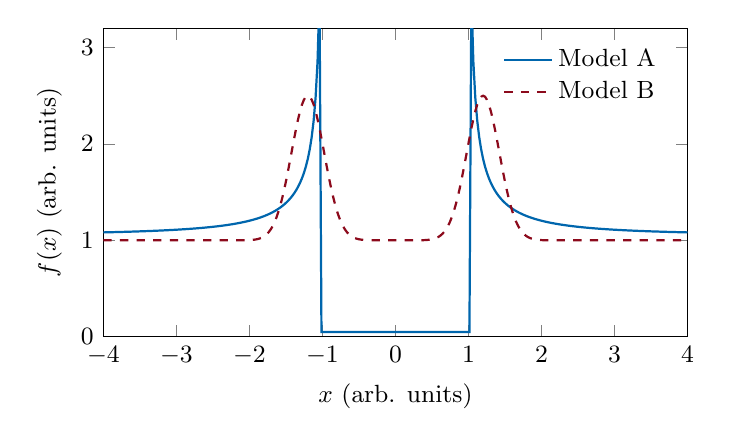
\begin{tikzpicture}
\begin{axis}[
    width=90mm, height=55mm,
    xlabel={$x$ (arb. units)}, ylabel={$f(x)$ (arb. units)},
    xmin=-4, xmax=4, ymin=0, ymax=3.2,
    legend pos=north east, legend cell align=left,
    legend style={draw=none, fill=none, font=\small},
    tick label style={font=\small}, label style={font=\small},
]
\addplot[c1, thick, domain=-4:4, samples=301]
    {abs(x)/sqrt(x^2 - 1 + 0.08^2 + 1e-9) * (abs(x) > 1.02) + 0.05};
\addlegendentry{Model A}
\addplot[c2, thick, dashed, domain=-4:4, samples=301]
    {1 + 1.5*exp(-(abs(x)-1.2)^2/0.1)};
\addlegendentry{Model B}
\end{axis}
\end{tikzpicture}
\end{document}
